\documentclass{article}
\usepackage{CJKutf8, indentfirst, graphicx, amsmath}
\begin{document}
\begin{CJK}{UTF8}{bsmi}
\title{硬體設計與實驗 Lab8 Report}
\author{104021219 鄭余玄}
\date{}
\maketitle
\section{實做過程}
這次 lab 主要是從助教的 demo2 程式碼去修改,除了輸入輸出訊號以外,只會改到 memory address generator,而且圖檔只需要重複使用助教提供的就行了,因此這次 lab 就非常快速就能完成了。 enable 訊號處理方式就如同以往的 lab,最後再判斷 dir 訊號和邊界條件,讓 position 加一或減一達到左右移動的效果(pixel\_addr 中的 position 沒有乘以 320 就可以左右移動)。此外,助教所使用的 clockdivisor,我還是重複利用之前的 clock\_divider 來產生,25 MHz 的訊號,也就是 $\frac{\text{clk}}{2^2}$,同樣可以使用參數化的寫法。

\subsection{Block diagram}
\begin{figure*}[h]
\centering{
    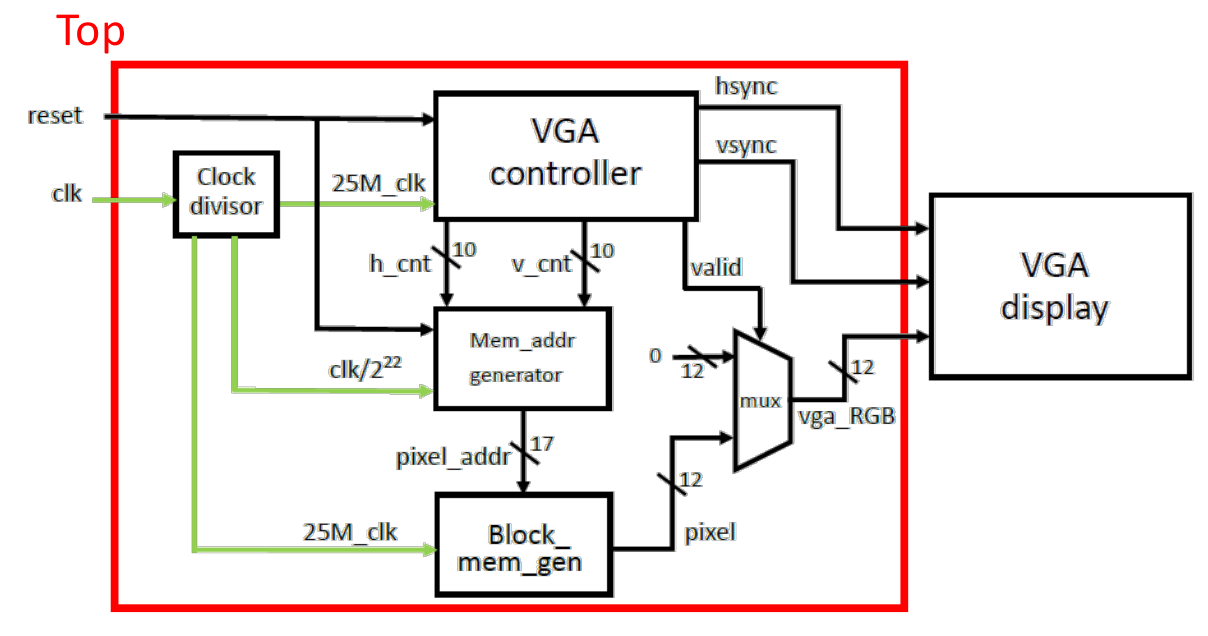
\includegraphics[width=.8\textwidth]{lab8}\label{fig:lab8}
}
\caption{Block diagram: demo2.}
\end{figure*}
這次 lab 的 Block diagram 其實和 demo2 差不多,所以就放 demo2 的。

\section{學到的東西及遇到的困難}
雖然以前就知道 CRT 運作原理,不過這次是第一次接觸到有 hsync 和 vsync 訊號實做的電路(雖然助教已經寫好了)。也是第一次知道會有一段 Blanking Time 讓電子槍緩衝,還有透過減少樣本點讓 artix7 的 RAM 可以塞的下圖片等技巧。這次基本上只有略改程式碼,因此沒有遇到特別的困難。

\section{想對老師或助教說的話}
覺得這次 lab 可以在多加一些控制項目,就像上次音樂盒 lab 一樣,可以切換圖片等等的,或是做幻燈片,這樣或許可以讓這次 lab 更豐富一點。

\end{CJK}
\end{document}
